%\chapter{Détection de sections et entités juridiques}
\chapter{Annotation des sections et entités juridiques}
\label{chap:structuration}

% court abstract
% Objectif: L'annotation manuelle peut atteirndre des interagréments raisonables (kappa) et nous démontrons qu'il est faisable d'automatiquement annoter les sections et métadonnées de référence d'un jugement à l'aide de modèle probabiliste graphiques comme le CRF ou le HMM moyennant de bien choisir les features
%Mots clés: annotation d'entités nommées judiciaires, chaine caché de markov, champ conditionnel aléatoires

\section{Introduction}
\label{sec:structuration:motivation}
Ce chapitre traite de la détection de sections et d'entités dans les décisions jurisprudentielles françaises. Bien qu'elles ne soient pas structurées, leur contenu est organisé en sections dont les principales : l'entête, le corps, et le dispositif. Chaque section décrit des informations spécifiques de l'affaire: 
\begin{itemize}
	\item l'entête contient de nombreuses méta-données de référence comme la date, le lieu, les participants etc.
	\item le corps détaille les faits, les procédures antérieures, les conclusions des parties et le raisonnement des juges;
	\item le dispositif est la synthèse du résultat final c'est-à-dire qu'on y retrouve les réponses aux demandes des parties.
\end{itemize}

Compte tenu de la répartition des informations, il nous a paru plus simple d'annoter au préalable les sections en segmentant le document. Par la suite, des données sur les entités ou les demandes par exemple peuvent être plus facilement extraites en fonction des sections où elles se retrouvent généralement. Nous nous focalisons en particulier ici sur la détection d'entités telles que la date à laquelle le jugement a été prononcé, le type de juridiction, sa localisation (ville), les noms de juges, des parties, et les règles de lois citées (normes). La Table \ref{tab:structuration:relevantinfo} liste les différentes entités ciblées et fournit des exemples illustrant la forme de leurs occurrences dans les décisions de cour d'appel.

\begin{table}[!ht]
\scriptsize
\begin{tabular}[c]{|p{0.17\textwidth}|c|p{0.37\textwidth}|cc|}
\hline
\textbf{Entités} & \textbf{Label} & \textbf{Exemples} & \multicolumn{2}{c|}{\textbf{\#mentions}$^a$}\\
  & & & \textbf{Médiane}$^b$& \textbf{Total}$^c$ \\ \hline
Numéro de registre général (R.G.) & \textbf{rg} & "10/02324", "60/JAF/09" & 3 & 1318\\ \hline
Ville & \textbf{ville}& "NÎMES", "Agen", "Toulouse" & 3 & 1304\\ \hline
Juridiction & \textbf{juridiction} & "COUR D'APPEL" & 3 & 1308\\ \hline
Formation & \textbf{formation} & "1re chambre", "Chambre économique" & 2 &  1245\\ \hline
Date de prononcé de la décision & \textbf{date} & "01 MARS 2012", "15/04/2014" & 3 & 1590\\ \hline
Appelant & \textbf{appelant} & "SARL K.", "Syndicat ...", "Mme X ..." & 2 & 1336 \\ \hline
Intimé & \textbf{intime} & - // - & 3 & 1933 \\ \hline
Intervenant & \textbf{intervenant} & - // - & 0 & 51 \\ \hline
Avocat & \textbf{avocat} & "Me Dominique A., avocat au barreau de Papeete" & 3 & 2313\\ \hline
Juge & \textbf{juge} & "Monsieur André R.", "Mme BOUSQUEL" & 4 & 2089\\ \hline
Fonction de juge & \textbf{fonction} & "Conseiller", "Président" & 4 & 2062\\ \hline
Norme & \textbf{norme} & "l' article 700 NCPC", "articles 901 et 903" & 12 & 7641 \\ \hline
%Argent & \textbf{argent} & "un euro", "" & 14$^*$ & 1777$^*$ \\ \hline
\noalign{\smallskip}\hline\noalign{\smallskip}
Non-entité & \textbf{O} & \textit{mot ne faisant partie d'aucune mention d'entité} & - & -\\ \hline
\end{tabular} 

$^a$ nombre de mentions d'entités dans le corpus annoté pour les expérimentations

$^b$ nombre médian de mentions par document dans le corpus annoté

$^c$ nombre total d'occurrences dans le corpus annoté

$^*$ Les statistiques sur les sommes d'argent ne concernent que 100 documents annotés (max=106, min=1, moyenne=17.77), contre 500 documents pour les autres entités.
\caption{Entités et labels correspondant utilisés pour labelliser leurs mots. }\label{tab:structuration:relevantinfo}
\end{table}

On s'attendrait à ce qu'une institution comme la justice respecte un modèle stricte et commun à tous les tribunaux pour la rédaction des décisions pour permettre de facilement les lire et les analyser. Malheureusement, même si les informations sont de même nature, le modèles employé semble varier entre les juridictions. C'est ce qu'on remarque déjà au niveau de l'enchainement des sections. Au vu de leur rôle, il est évident que les sections devraient être séparées par des marqueurs bien précis. Une approche intuitive de sectionnement consisterait par conséquent à définir un algorithme capable de reconnaître ces marqueurs de transitions à travers des expressions régulières. Cependant, les marqueurs utilisés ne sont pas standards car il n'existe pas de modèle stricte utilisé par toutes les juridictions. par conséquent, les marqueurs de transitions sont souvent différents d'une décision à l'autre et peuvent être des titres ou des motifs à base de symboles (astérisques, tirets, etc.). Il arrive parfois que la transition soit implicite et qu'on ne s'en rende compte que par la forme des lignes, au cours de la lecture. Même les marqueurs explicites sont hétérogènes. D'une part en cas d'utilisation de titres par exemple, la transition de l'entête à l'exposé du litige peut être indiquée par des titres comme "\textit{Exposé}", "\textit{FAITS ET PROCÉDURES}", "\textit{Exposé de l'affaire}", "\textit{Exposé des faits}", etc. Quant au dispositif, il est introduit généralement par l'expression "\textit{PAR CES MOTIFS}" avec souvent quelques variantes qui peuvent être très simples (par ex. "\textit{Par Ces Motifs}") ou exceptionnelles (par ex. "\textit{P A R C E S M O T I F S :}"). Dans certaines décisions, cet expression est remplacée par d'autres expressions comme "\textit{DECISION}", "\textit{DISPOSITIF}", "\textit{LA COUR}", etc. 
D'autre part lors de l'utilisation de symboles, il arrive qu'un même motif sépare différentes sections et même des paragraphes dans le même document. Une différence similaire apparaît pour les entités. Les noms de parties et d'avocats sont généralement placés après un mot particulier comme  "\textit{APPELANTS}" ou "\textit{DEMANDEUR}" pour les demandeurs (appelants en juridiction de 2e degré), "\textit{INTIMES}" ou "\textit{DEFENDEUR}" pour les défendeurs (ou intimés), and "\textit{INTERVENANTS}" pour les intervenants. Les noms des individus, sociétés et lieux commencent par une lettre majuscule ou sont entièrement en majuscule. Cependant, certains mots communs peuvent apparaître aussi en majuscule (par ex. \textit{APPELANTS}, \textit{DÉBATS}, \textit{ORDONNANCE DE CLÔTURE}). Les entités peuvent contenir des chiffres (identifiant, dates, ...), des caractères spéciaux ("/", "-"), des initiaux ou abréviations.  Dans l'entête, les entités apparaissent généralement dans le même ordre (par ex. les appelants avant les intimés, les intimés avant les intervenants). Cependant, plusieurs types d'entités apparaissent dans l'entête, contrairement aux autres sections où seules les normes nous intéressent dans cette étude. L'entête est aussi mieux structurée que les autres sections même si sa structure peut différer entre deux documents.

Notre étude consiste à analyser l'application du Modèle Caché de Markov (HMM) et des Champs Aléatoires Conditionnels (CRF) pour le sectionnement et la reconnaissance d'entités juridiques. Ces deux tâches sont ainsi représentées sous forme d'un problème d'étiquetage de séquence. L'idée est de segmenter un texte en des segments atomiques (\textit{token}) qui peuvent être des mots, des phrases, des paragraphes, etc. Le texte est ainsi représenté sous forme de séquence et chaque objet d'intérêt (section ou entité) comprend  un ou plusieurs éléments. Un label est défini pour chaque type d'entité (par ex. PER pour les noms de personnes). Considérons un texte $T$ comme étant une séquence d'observations $t_{1:n}$, avec chaque $t_i$ étant un segment de texte (mots, ligne, phrase, etc.). En considérant une collection de labels, l'étiquetage de $T$ consiste à affecter à les labels appropriés à chaque $t_i$. La segmentation de $T$ est un étiquetage particulier qui implique de découper $T$ en des groupes qui ne se chevauchent pas (des partitions), tels que les segments d'un groupe constituent nécessairement une sous-séquence de $T$. En d'autres termes, segmenter $T$ revient à labelliser ses segments en considérant une contrainte particulière. 


\section{Détection d'information par étiquetage de séquence}
\label{sec:structuration:biblio}

\citet{chau2002nerwithNN} distinguent quatre catégories d'approches de détection d'entités :

\begin{itemize}
\item Les \textbf{systèmes à recherche lexicale} sont conçus sur la base d'une liste d'entités précédemment connues, avec leurs synonymes dans le domaine d'intérêt. Par exemple, dans le domaine juridique, un lexique pourrait contenir les identifiant de règles juridiques et les noms des juges. La liste des entités peut être manuscrite par des experts ou apprise à partir d'un ensemble de données étiquetées (phase d'apprentissage). Cependant, il s'avère très difficile de maintenir une telle liste car le domaine pourrait changer régulièrement (nouvelles lois par ex.). De plus, les mentions d'entités peuvent avoir plusieurs variantes. Par exemple, la même règle "Article 700 du code de procédure civile" peut être citée seule et en entier (\textit{article 700 du code de procédure civile}), ou abrégée (\textit{article 700 CPC}), ou encore combinée avec d'autres règles (\textit{articles 700 et 699 du code de procédure civile}). Ces problèmes, y compris les ambiguïtés (par exemple, différentes entités utilisant les mêmes mots), ont limité les premiers systèmes \citep{palmer1997learnedLookup}.

\item Les \textbf{systèmes à base de règles} décrivent suffisamment la diversité des mentions d'entités en fonction de la régularité du contexte, de la structure et du lexique. Ils sont avantageux parce que leurs erreurs sont facilement explicables. La définition manuelle de règles exige malheureusement des efforts considérables, en particulier pour les grands corpus. De plus, un ensemble donné de règles est difficilement réutilisable dans d'autres domaines. Cependant, quelques approches adaptatives ont été conçues pour surmonter ces limites tout en bénéficiant toujours de facilité à expliquer le comportement des systèmes à base de règles \citep{siniakov2008gropusrulebased,chiticariu2010adaptativerulebased}.

\item Les \textbf{systèmes statistiques} adaptent les modèles statistiques de langage, issus typiquement des méthodes de compression de texte, pour détecter les entités. Par exemple, \citet{witten1999languagemodel} ont adapté les schémas de compression nommés "Prédiction par Correspondance Partielle".

\item Les \textbf{systèmes basés sur l'apprentissage automatique} exécutent des classifieurs multi-classes sur des segments de texte. Par exemple, un classifieur traditionnel comme le classifieur bayésien naïf peut être entraîner pour détecter les noms de gènes en classifiant les mots du documents à partir d'un ensemble de descripteurs définis manuellement \citep{persson2012nbbioner}. Pour détecter les entités, les algorithmes d'étiquetage de séquence tels que le CRF quant à eux classifient les segments de texte tout en modélisant les transitions entre les labels \citep{finkel2005stanfordcrfner}. Dans ce registre, les architectures d'apprentissage profond réalisent actuellement les meilleures performances sur de multiples tâche d'extraction d'information en général et de reconnaissance d'entités nommées en particulier \citep{lample2016nnner}.
\end{itemize}
Certains travaux ont combiné différentes approches pour extraire les entités à partir de documents juridiques,  par exemple,  par la description de l'information contextuelle en utilisant des règles pour répondre au problème d'ambiguïté des méthodes à recherche lexicale \citep{mikheev1999NERlexicalWithRules,hanisch2005prominer}. 

La comparaison avec d'autres approches démontre bien que les modèles probabilistes atteignent de très bonnes performances lors de l'extraction d'information dans les documents juridiques. Par exemple, le HMM a été comparé à l'Algorithme de Perceptron à Marges Inégales (PAUM) \citep{li2002PAUM} pour reconnaître les institutions et références d'autres décisions de justice, ainsi que les citations d'actes juridiques (loi, contrat, etc.) dans les décisions judiciaires de la République Tchèque \citep{Kriz2014nerinczechdecisions}. Les deux modèles ont données de bonnes performances avec des scores F1 de $ 89 \% $ et $ 97 \% $ pour le HMM utilisant les trigrammes comme descripteurs de mots, et des scores F1 de $ 87 \% $ et $ 97 \% $ pour le PAUM en utilisant des 5-grammes de lemmes et les rôles grammaticaux (\textit{Part-Of-Speech tag}) comme descripteurs. 


\subsection{HMM}
Un modèle HMM est une machine à état fini défini par un ensemble d'états $ \lbrace s_1, s_2, ..., s_m \rbrace $. Un modèle HMM a pour fonction d'affecter une probabilité jointe 
$ P (T , L) = \prod\limits_i P(l_i \vert l_{i-1})P(T \vert l_i)$  à des paires de séquences d'observations $ T = t_{1: n} $ et de séquence de labels $ L = l_{1:n} $. Étant donnée qu'un HMM est un modèle génératif, chaque label $l_i$ correspond à l'état $s_j$ dans lequel la machine a généré l'observation $t_i$. Il y a autant de labels possibles que d'états. Le processus de labellisation de T consiste à déterminer la séquence de labels $ L^* $ qui maximise la probabilité jointe ($L^* = \arg \max\limits_L P(T, L)$). Une évaluation de toutes les séquences possibles de labels est nécessaire pour déterminer celle qui convient mieux à $ T $. Pour éviter la complexité exponentielle $ O(m^n)$ d'une telle approche, $n$ étant la longueur de la séquence et $m$ le nombre de labels possibles, le processus d'étiquetage utilise généralement l'algorithme de décodage Viterbi \citep{viterbi1967viterbi} qui est basé sur la programmation dynamique. Cette algorithme utilise les paramètres du HMM estimés par apprentissage sur un corpus de textes annotés manuellement:
\begin{itemize}
\item Un ensemble d'états $ \lbrace s_1, s_2, ..., s_m \rbrace $ et un alphabet $ \lbrace o_1, o_2, ..., o_k \rbrace $
\item La probabilité que $ s_j $ génère la première observation $ \pi(s_j), \forall j \in [1 .. m] $
\item La distribution de probabilité de transition $ P (s_i\vert s_j),  \forall i,j \in [1 .. m] $
\item La distribution de probabilité de d'émission $ P(o_i\vert s_j), \forall i \in [1 .. k], \forall j \in [1 .. m]$
\end{itemize}

Les probabilités de transition et d'émission peuvent être inférer en utilisant une méthode de maximum de vraisemblance comme l'algorithme d'espérance maximale. L'algorithme Baum-Welch \citep{welch2003baumwelch} en est une spécification conçue spécialement pour le HMM. L'avantage du HMM réside dans sa simplicité et sa vitesse d'entraînement. Par ailleurs, il est difficile de représenter de multiples descripteurs interactifs pour les segments de texte, tout comme de modéliser la dépendance entre des observations distantes parce que l'hypothèse d'indépendance entre observations est très restrictive (i.e. l'état courant dépend uniquement des état précédents et de l'observation courante). \citet{rabiner1989tutorial} fournit plus de détails sur le HMM.

\subsection{CRF}
\label{sec:structuration:biblio:CRF}

Même si l'algorithme Viterbi est aussi utilisé pour appliquer le CRF à l'étiquetage de séquence, les structures du CRF et du HMM diffèrent. Au lieu de maximiser la probabilité jointe $ P(L, T)$ comme le HMM, un CRF \citep{lafferty2001crfie} cherche la séquence de labels $L^*$ qui maximise la probabilité conditionnelle suivante: $$P(L|T) = \frac{1}{Z}\exp \left(\sum\limits_{i=1}^n\sum\limits_{j=1}^F \lambda_j f_j(l_{i-1},l_i,t_{1:n},i)\right)$$ où $Z$ est le facteur de normalisation. Les fonctions potentielles $f(\cdot)$ sont les caractéristiques utilisés par les modèles CRF. Deux types de fonctions caractéristiques sont définies: les caractéristiques de transition qui dépendent des labels aux positions courantes et précédentes ($l_{i-1}$ et $ l_{i}$ respectivement) et de $T$; et les caractéristiques d'état qui sont des fonctions de l'état courant $ l_{i} $ et de la séquence $ T $. Ces fonctions $f(\cdot)$ sont définies à l'aide soit par de fonctions à valeur binaire ou réelle $b(T,i)$ qui combine les descripteurs d'une position $i$ dans $T$ \citep{Wallach2004crfintro}. Pour labelliser les références aux règles de loi par exemple, un CRF pourrait inclure par exemple les fonctions potentielles pour labelliser "\textit{700}" dans ce contexte "\textit{... l'article 700 du code de procédure civile...}":
{%\scriptsize
\[f_1(l_{i-1},l_i,t_{1:n},i) = \left\lbrace \begin{array}{ll}
b_1(T,i) & \text{si } l_{i-1} = \text{NORME} \wedge l_i = \text{NORME} \\
0 & \text{otherwise}
\end{array} \right.\]
\[f_2(l_{i-1},l_i,t_{1:n},i) = \left\lbrace \begin{array}{ll}
b_2(T,i) & \text{si }l_i = \text{NORME} \\
0 & \text{otherwise}
\end{array} \right.\]
avec
\[b_1(T,i) = \left\lbrace \begin{array}{ll}
1 & \text{si } (t_{i-1} =\text{article) }\wedge (POS_{i-1}=\text{NOM}) \\&  \wedge  (NP1_{i-1}=\text{<unknown>)} \wedge (NS1_{i-1}=\text{@card@)} \\
0 & \text{otherwise} 
\end{array} \right.\]
\[b_2(T,i) = \left\lbrace \begin{array}{ll}
1 & \text{si } (t_i =\text{700) }\wedge (POS_i=\text{NUM})  \wedge (NP1_i=\text{article)} 
\wedge (NS1_i=\text{code)} \\
0 & \text{otherwise}
\end{array} \right.\]
}
$t_i$ étant une observation dans $T$, \verb|POS| étant le rôle grammatical de $t_i$ (\textit{NUM} = valeur numérique, \textit{NOM} = nom), et \verb|NP1| et \verb|NS1| sont les lemmes des mots avant et après $t_i$, respectivement. Les symboles \textit{<unknown>} et \textit{@card@} encode les lemmes inconnus et ceux des nombres respectivement. Pouvant être activées au même moment, les fonctions $f_1$ et $f_2$ définissent des descripteurs se chevauchant. Avec plusieurs fonctions activées, la croyance dans le fait que $l_i = NORME$ est renforcée par la somme $\lambda_1 + \lambda_2$ des poids  des fonctions activées \citep{Zhu2010CRFlecture}.  Un modèle CRF emploie une fonction $f_j$ lorsque ses conditions sont satisfaites et $\lambda_j > 0$. Les diverse fonctions pondérées $f_j$ sont définies par des descripteurs caractérisant le texte et les labels des données d'entraînement. La phase d'entraînement consiste principalement à estimer le vecteur de paramètres $\lambda = (\lambda_1,...,\lambda_F)$ à partir des de textes annotés manuellement $ \lbrace (T_1, L_1), ..., (T_M, L_M) \rbrace $, $ T_k $ étant un texte et $ L_k $ la séquence de labels correspondants. La valeur optimal retenue pour estimer de $\lambda$ est celle maximisant la fonction objectif   
$\sum\limits_ {k = 1} ^ M \log P (L_k \vert T_k) $ sur les données d'entraînement. En général, outre le maximum de vraisemblance, cette optimisation est résolue à l'aide de l'algorithme de descente du gradient dont l'exécution peut-être accélérée à l'aide de l'algorithme L-BFGS \citep{liu1989l-bfgs}.

\subsection{Représentation des segments atomiques}
%\textcolor{red}{Pourquoi? Quoi ? et Comment?}

La représentation des éléments atomiques occupe une place importante dans le bon fonctionnement des modèles  précédemment décrits. Elle permet de décrire la forme et le contexte du segment. Le principe consiste généralement à assigner à chaque segment des attributs qui peuvent prendre différentes formes \citep{nadeau2007nersurvey,sharnagat2014nersurvey}. Elles peuvent être booléennes (\og le mot est il en majuscule? \fg{}), numériques (nombre de caractères du mot), nominales (par ex. le rôle grammatical d'un mot), ou à base d'expressions régulières (par ex. pour les numéros R.G. on aurait \verb|dd/ddddd| où \verb|d| désigne un chiffre). Ces descripteurs mettent  en évidence des caractéristiques particulières des différents types d'entités. Par exemple, préciser qu'un mot débute par une lettre majuscule permet d'indiquer les noms propres. La définition de tels descripteurs consiste ainsi à fournir au modèle des indices l'aidant à mieux distinguer les différents types d'entités par la forme et le contexte d'occurrence des éléments atomiques. 

Etant donné que les descripteurs dépendent généralement de l'intuition du modélisateur, il est difficile mais nécessaire d'identifier des descripteurs appropriés. Après avoir défini des candidats, il n'est pas sûr qu'en les combinant tous ensemble, on obtienne les meilleures performances. Une sélection de caractéristiques peut par conséquent s'avérer nécessaire. Cette sélection peut améliorer les performances d'étiquetage, d'accélérer les phases d'extraction de caractéristiques, d'entraînement et de prédiction, et de fournir une meilleure compréhension du comportement des modèles \citep{kitoogo2007featureSelectNER, klinger2009FeaturefilterCRF}. Deux principales approches se distinguent. Les méthodes \og filtrantes \fg{} (\textit{filters}), comme l'information mutuelle, comparent individuellement les descripteurs à l'aide de scores qui ne sont pas nécessairement basés sur la performance. Tandis que les méthodes \og enveloppantes \fg{} (\textit{wrappers}) comparent des sous-ensembles de descripteurs sur la base de leur performance. Même si les méthodes filtrantes sont plus rapides, elles sont moins performantes car elles ne permettent pas d'éviter les redondances, et ne prennent pas en compte l'effet de la combinaison de caractéristiques.
%. Au départ proposés et utilisés en classification multi-dimensionnelle, les algorithmes de sélections de caractéristiques ont été appliqués avec succès pour l'extraction d'entités. \citet{klinger2009FeaturefilterCRF} ont 

La définition manuelle des caractéristiques suivie de la sélection est souvent qualifiée de méthode forcée car elle dépend fortement de la capacité du concepteur du système à identifier les descripteurs appropriés. Les réseaux de neurones permettent d'apprendre des caractéristiques plus pertinentes grâce à des méthodes de plongement sémantique telles que Word2Vec \citep{lemikolov2014word2vec} et Glove \citep{pennington2014glove}.  Deux architectures de réseaux de neurones réalisent actuellement les meilleures performances en matière de détection d'entités nommées. Il s'agit du modèle LSTM-CRF de  \citet{lample2016nnner} et du LSTM-CNN-CRF de \citet{ma2016lstm-cnns-crf}. On pourrait résumer ces architectures en trois phases. Dans un premier temps, les segments de textes (mots) ont une représentation vectorielle concaténant 2 vecteurs de plongement sémantique: l'un issu de l'apprentissage morphologique du mot à partir de ces caractères, et l'autre issu de l'apprentissage du contexte général d'occurrence du mot. Lors de la seconde phase, deux couches de cellules LSTM enchaînées permettent de modéliser le contexte à droite et à gauche de chaque mots du texte. La dernière phase détermine la séquence de label la plus probable pour le texte à l'aide d'une implémentation d'un modèle CRF sous forme de réseau de neurones. Le CRF reçoit en entrée la concaténation des contextes à droite et à gauche des mots.

%2015 https://arxiv.org/pdf/1508.01991.pdf
%https://github.com/UKPLab/emnlp2017-bilstm-cnn-crf
%dnn crf : https://pdfs.semanticscholar.org/c322/7702dd212965157a615332f3dd78b0f11b5e.pdf
%https://towardsdatascience.com/conditional-random-field-tutorial-in-pytorch-ca0d04499463

\subsection{Schéma d'étiquetage}
Nous traitons d'entités dont les occurrences comprennent un ou plusieurs éléments atomiques. Pour améliorer les performance d'un modèle d'étiquetage, certaines parties des entités peuvent être mise en évidence à travers une représentation appropriée de segment. Nous comparons dans cette étude quelques schémas d'étiquetage dont certains sont décrits par \citet{konkol2015tagModel}. Le schéma IO utilisé par défaut ne met l'accent sur aucune partie de l'entité et affecte le même label à chaque segment. D'autres schémas distinguent soit le premier élément (BIO), soit le dernier (IEO), soit les deux (BIEO). Les schémas IEO et BIO ont des variantes IEO1, BIO1, IOE2, et BIO2. IOE2, et BIO2 utilisent resp. les préfixes E- et B- pour étiqueter les entités à mot unique, contrairement à IEO1 et BIO1 qui utilisent plutôt le préfixe I-. Le modèle BIEO est souvent étendu à BIESO (ou BILOU) dans le cas où on souhaite distinguer les entités à un seul segment (par ex. ville ou numéro RG). Les lettres des sigles de ces modèles servent de préfixes aux labels et portent la signification suivante:

\begin{itemize}
\item B - "\textit{beginning}": début;
\item I - "\textit{inside}": intérieur;
\item E (ou L, ou M) - "\textit{end}" ou "\textit{last}" ou "\textit{middle}": fin;
\item S (ou U, ou W) - "\textit{single}" ou "\textit{unit}" ou "\textit{whole}": singleton;
\item O - "\textit{outside}": hors de toute entité.
\end{itemize}

La figure \ref{p4_sample-tagmod} illustrate l'utilisation des ces différents modèles sur un extrait de décision de justice:
\begin{figure}[!h]
\tiny
\begin{tabular}{l|ccccccccccc}
 & \textit{composée} & \textit{de} & \textit{Madame} & \textit{Martine} & \textit{JEAN} & , & \textit{Président} & \textit{de} & \textit{chambre} & , & \textit{de} \\ 
IO & O & O & I-JUGE & I-JUGE & I-JUGE & O & I-FONCTION & I-FONCTION & I-FONCTION & O & O \\
BIO & O & O & B-JUGE & I-JUGE & I-JUGE & O & B-FONCTION & I-FONCTION & I-FONCTION & O & O \\
IEO & O & O & I-JUGE & I-JUGE & E-JUGE & O & I-FONCTION & I-FONCTION & E-FONCTION & O & O \\
BIEO & O & O & B-JUGE & I-JUGE & E-JUGE & O & B-FONCTION & I-FONCTION & E-FONCTION & O & O \\
\end{tabular}
\caption{Illustration de différents schémas d'étiquetage}\label{p4_sample-tagmod}
\end{figure}

Il est possible d'aller plus loin en mettant l'accent sur les mots avant  (O-JUGE) et après (JUGE-O) l'entité (JUGE par exemple) et en indiquant le début (BOS-O, \textit{begininning of sentence}) et la fin (O-EOS, \textit{end of sentence}) du texte. Le format ainsi obtenu est appelé BMEWO+ \citep{baldwin2009bmewo}.

Un autre intérêt très important de modèle plus complexes que IO est de pouvoir distinguer des entités qui se suivent sans être séparées d'une ponctuation visible. Cet aspect est notamment important dans les décisions de justice par exemple lorsque des noms de parties sont listés dans la section ENTETE en n'étant séparés que d'un simple retour à la ligne (\textcolor{red}{Illustration?}).

\section{Architecture proposée}
\label{sec:structuration:proposition}
\begin{figure}[!h]
%\sidecaption
\centering
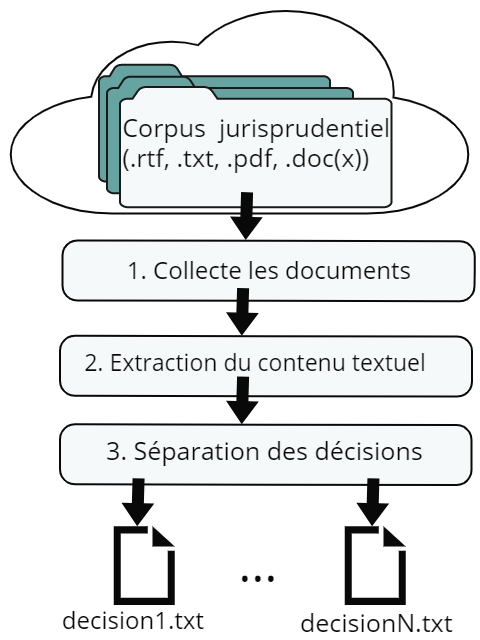
\includegraphics [width=0.45\textwidth]{structuration-preprocess.png}
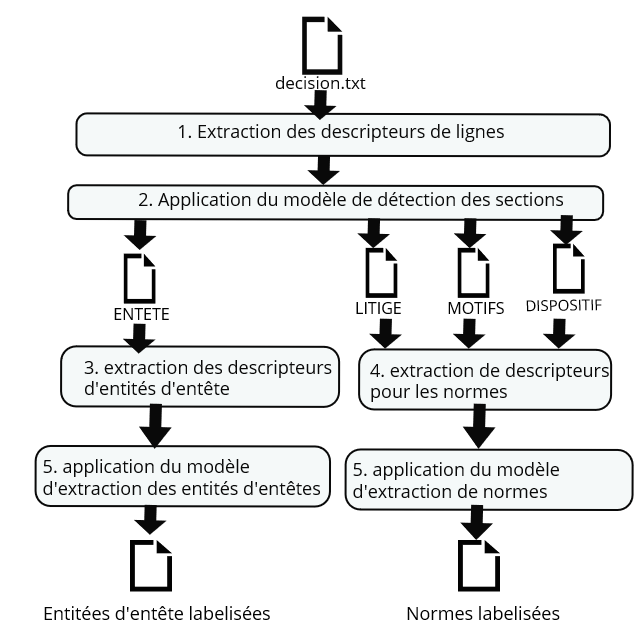
\includegraphics [width=0.45\textwidth]{structuration-pipeline-application.png}

{\scriptsize Après la collecte et le prétraitement des documents, l'étiqueteur de ligne est d'abord appliqué pour détecter les sections, puis les étiqueteurs d'entités peuvent être appliqués simultanément dans différentes sections.}
\caption{Application des modèles entraînes d'étiquetage de section et entités.}\label{p4_archAppli}
\end{figure}
Nous proposons de travailler uniquement avec le contenu textuel des documents. Ce contenu est extrait des documents téléchargés en éliminant les éléments inutiles, principalement des espaces vides. Ces éléments sont typiques des documents formatés (\verb|.rtf, .doc(x), .pdf|). Ils ne fournissent pas une indication standard sur le début des sections. Le choix de ne pas exploiter le formatage des documents permet d'avoir à gérer un nombre plus faible de diversités entre les textes tout appliquant le même processus de traitement à tout document indépendamment de sont format d'origine. Une simple architecture d'étiquetage de sections et d'entités juridiques a été conçu avec cet uniformisation des documents comme point d'entrée. Ainsi, les documents sont collectés puis pré-traités suivant leur format d'origine (extraction du texte et séparation des décisions apparaissant dans le même document).  Ensuite, après le sectionnement des décisions, les entités sont identifiées dans les différentes sections. Par ailleurs, Comme segment atomique à étiqueter nous avons choisi les lignes pour la détection des sections, et les mots pour les entités. 

\begin{figure}[!h]
%\sidecaption
\centering
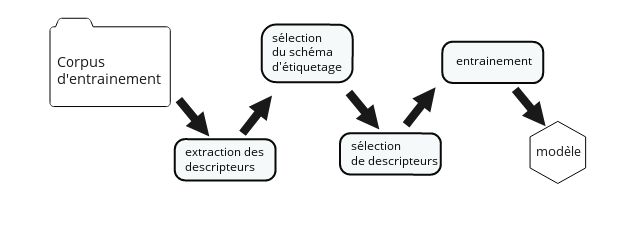
\includegraphics [width=\textwidth]{structuration-training.png}
\caption{Entrainement des modèles.}\label{fig:structuration:training}
\end{figure}


Les modèles HMM et CRF étant tous les deux supervisés, ils doivent être entraînés sur des exemples manuellement annotés pour estimer leurs paramètres. Nous proposons de sélectionner le schéma d'étiquetage et les sous-ensembles minimaux de caractéristiques manuellement définies, avant d'entraîner les modèles HMM et CRF (Figure \ref{fig:structuration:training}). 

\subsection{Définition de descripteurs candidats}

\subsubsection{Descripteurs candidats pour la détection des sections}

Nous considérons donc la ligne comme élément à étiqueter lors du sectionnement. Nous n'avons pas travailler au niveau des mots afin d'éviter que des mots de la même ligne ne soient classés dans des sections différentes. L'étiquetage des phrases a été aussi évité car en découpant les documents en phrases tel qu'elles sont comprises en français, on a généralement des segments qui s'étendent d'une section à une autre (absence de ponctuation), et de plus, l'entête en particulier a plus l'apparence d'un formulaire.

Plusieurs critères peuvent être utilisés pour différencier les sections, à savoir: la longueur des lignes (plus longues dans le corps, plus courtes dans l'en-tête), les premiers termes de certaines lignes (typiques de chaque section) et le nombre total de lignes. Un HMM n'adapte qu'un descripteur assimilé à l'élément à étiqueter. D'autres descripteurs peuvent être la position de l'élément à étiqueter (numéro de ligne) ou le début de la ligne. Une entité capturant la longueur de ligne peut être absolue (nombre exact de mots dans la ligne) ou relative, en fonction de la catégorisation de la longueur de ligne. Sur la base des quantiles de distribution de longueur de ligne sur un ensemble de décisions, nous avons défini trois catégories:
\verb|LQ1| ($longueur \leq$ 5), \verb|LQ2| (5 < $longueur \leq$ 12) et \verb|LQ2| (12 < $longueur \leq$ 14). Nous avons également catégorisé les parties de documents afin de capturer une position de ligne relative.

Lors de l'extraction des caractéristiques, le document est considéré comme divisé en $N$ parties (10 dans nos expériences). La position relative d'une ligne est donc le numéro de la partie contenant la ligne particulière. En résumé, les caractéristiques sont décrites comme suit (avec leurs étiquettes entre parenthèses):
\begin{itemize}
 \item forme de la ligne: la ligne entière, ses premiers mots (\verb|t0, t1, t2|), sa longueur absolue (\verb|absLength|) et sa longueur relative (\verb|relLength|);
 \item contexte de ligne: le numéro de ligne (\verb|absNum|) et le numéro de la partie de document contenant la ligne (\verb|relNum|), les deux premiers mots des lignes précédente (\verb|p0, p1|) et suivantes (\verb|n0, n1|), ainsi que leurs valeurs absolues respectives. longueurs relatives
 (\verb|pLength|, \verb|pRelLength|, \verb|nLength|, \verb|nRelLength|).
\end{itemize}

\subsubsection{Descripteurs candidats pour la détections d'entités}

La détection d'entité consiste à former soit un CRF, soit un HMM pour étiqueter les différentes entités (mot, ponctuation, numéro, identifiant). Les deux modèles nécessitent des caractéristiques, dont certaines peuvent être défini sur la base de motifs directement observables dans les textes. Il est également possible d'obtenir des descripteurs à partir du résultat d'autres tâches d'analyse de texte.

Sur la base des observations de décision, nous avons défini les caractéristiques suivantes basées sur l'orthographe pour les mots des deux normes.
entités dans les en-têtes (avec leurs noms entre parenthèses):
\begin{itemize}
	\item forme du mot: le mot (\verb|token|), son lemme (\verb|lemma_W0|), "Commence-t-il par une lettre majuscule?" (\verb|startsWithCAP|), "est-il entièrement capitalisé?" (\verb|isAllCAP|), "est-ce une initiale solitaire?" comme par exemple "B." (\verb|isLONELYINITIAL|), "contient-il un caractère de ponctuation?" (\verb|PUN-IN|), "est-ce toute la ponctuation?" (\verb|isALLPUN|), "contient-il un caractère numérique?" (\verb|DIGIT-IN|), "y a-t-il juste tous les chiffres?" (\verb|isALLDIGIT|);
	\item contexte de mot: les mots précédents (\verb|w-2, w-1|) et suivants (\verb|w1, w2|) et leurs lemmes (\verb|lemmaW|$_i$). La lemmatisation homogénéise les variantes du même mot. Les mots adjacents sont choisis pour indiquer les termes couramment utilisés pour introduisent des entités.
\end{itemize}

Plus particulièrement pour les en-têtes, nous avons défini des descripteurs supplémentaires pour capter le contexte du mot: numéro de ligne (\verb|lineNum|), position de l'élément dans la ligne (\verb|numInLine|), "le texte contient-il le mot clé intervenant?" (\verb|intervenantInText|), le texte vient-il après le mot clé "APPELANT" (\verb|isAfterAPPELANT|), "INTIME" (\verb|isAfterINTIME|), "INTERVENANT" (\verb|isAfterINTERVENANT|). Nous avons également pris en compte les dernières lignes, où le mot était précédemment rencontré dans le texte ( \verb|lastSeenAt| ), ainsi que le nombre de fois où il a été trouvé ( \verb|nbTimesPrevSeen| ), car les noms des parties sont souvent répétés à des emplacements différents. Nous avons également défini une caractéristique spéciale pour les normes: "le mots est-il un mot clé de règles juridiques?" (\verb|isKEYWORD|). Pour ce dernier descripteur, nous avons établi une courte liste de mots-clés généralement utilisés pour citer des règles juridiques (article, code, loi, contrat, décret, convention, civil, pénal, etc.).

Nous avons étendus ces caractéristiques avec les rôles grammaticaux (\textit{Part-of-Speech} et les modèles thématiques (\textit{topic model}).

\textbf{Rôles grammaticaux}: Certaines entités ont tendance à contenir des rôles grammaticaux particuliers. Par exemple, les noms des
les individus sont composés de noms propres (Chang et Sung, 2005). Nous avons extrait le rôle grammatical du mot courant (\verb|POS|) ainsi que celui de ses voisins (\verb|POSW-2, POSW-1, POSW1, POSW2|).

\textbf{Modèles thématiques}: comme \citet{polifroni2011usingLDA} et \citet{nallapati2010blinddomaintransferner}, nous utilisons des associations de mot-thème pour décrire les mots. Il s'agit de modéliser un ensemble de N thèmes et d'utiliser leurs identifiants comme fonctionnalités. Il serait peut-être intéressant d'utiliser la probabilité déduite du modèle thématique, mais l'inférence sous-jacente au modèle LDA \citep{blei2003lda} n'est pas déterministe (la distribution de probabilité change pour le même mot entre différentes inférences).
Néanmoins, l'ordre des sujets ne changeant pas de manière significative, nous avons utilisé l'ID du mot le plus pertinent (\verb|topic0|) ainsi que celui de ses voisins (\verb|w-2topic0|, \verb|w-1topic0|, \verb|w1topic0|, \verb|w2topic0|).

\subsection{Sélection des descripteurs}
\subsubsection{Descripteurs pour le modèle CRF}
 Nous avons étudié deux approches enveloppantes qui semblent toujours converger et qui ne nécessitent pas de définir manuellement la taille du sous-ensemble cible. Il s'agit de la recherche bidirectionnelle et de la  sélection séquentielle à flottement avant.

La recherche bidirectionnelle (BDS), de \citet{liu2012featureSelection}, combine la sélection séquentielle en avant (SFS) et la sélection séquentielle en arrière (SBS) en parallèle. La SFS recherche un sous-ensemble optimal, en commençant par un ensemble vide et en ajoutant le descripteur qui améliore le mieux la performance du sous-ensemble sélectionné. Le critère de performance dans notre cas est définie par la F1-mesure (Eq. \ref{eq:structuration:f1mesure}). Contrairement à la SFS, la SBS commence par l'ensemble des candidats et supprime successivement les plus mauvais descripteurs. Les caractéristiques ajoutées par la SFS ne doivent pas être celles déjà supprimées par la SBS. Le principe de la recherche bidirectionnelle BDS est décrite par l'Algorithme \ref{algo:structuration:bds}.

\begin{algorithm}[H]
\KwData{Données annotées, $X$ liste de tous les descripteurs candidats}
\KwResult{Sous-ensemble optimal de descripteurs}
	Démarrer la SFS avec $Y_{F_0}= \emptyset $\; 
	Démarrer la SBS avec $Y_{B_0}=X$\; $k=0$\;
	\While{$Y_{F_k} \neq Y_{B_k}$}{
		$x^+=\argmax_{\substack{x \in Y_{B_k} \setminus Y_{F_k}}} F1measure(Y_{F_k} + x)$\;
		$Y_{F_{k+1}} = Y_{F_k} + x^+$\;
		$x^-=\argmax_{\substack{x \in Y_{B_k} \setminus Y_{F_{k+1}}}} F1measure(Y_{F_k} - x)$\;
		$Y_{B_{k+1}} = Y_{B_k} - x^-$\; 
		$k = k+1$;
	}
	\Return $Y_{F_k}$\;
	\caption{Recherche bidirectionnelle BDS} \label{algo:structuration:bds}
\end{algorithm}

L'algorithme de sélection séquentielle avant à flottement SFFS (Algorithme \ref{algo:structuration:sffs}) de \citet{pudil1994floatingFeatSelection} corrigent leur limitation séparément. Pour surmonter l'incapacité de l'algorithme SFS à réévaluer l'utilité d'un descripteur après son rejet, le SFFS effectue des étapes en arrière à chaque étape. 

\begin{algorithm}[H]
	\KwData{Données annotées, $X$ liste de tous les descripteurs candidats}
	\KwResult{Sous-ensemble optimal de descripteurs}
	$Y_0= \emptyset $\; 
	$k=0$\;
	\Repeat{$X = \emptyset$ ou $X = Y_{k}$}{
		$x^+=\argmax_{x \notin Y_k} F1(Y_k + x)$\; \label{p4_forward_sffs}
		$Y_k = Y_k + x^+$\; 
		$x^-=\argmax_{x \in Y_k} F1(Y_k - x)$\; \label{p4_back_sffs}
		\eIf{F1($Y_k - x^-$) > F1($Y_k$)}{
			$Y_{k+1} = Y_k - x^-$\; 
			$X = X - x^-$\;
			$k = k+1$\;
			Rentrer à \ref{p4_back_sffs}\;
		}{
			Rentrer à  \ref{p4_forward_sffs}\;
		}
	}
	\Return $Y_k$\;
	\caption{Sélection séquentielle avant à flottement}\label{algo:structuration:sffs}
\end{algorithm}

\subsubsection{Descripteurs pour le modèle HMM} Pour sélectionner les meilleurs descripteurs pour les modèles HMM, nous avons testé individuellement les différents candidats. La caractéristique donnant le meilleur résultat sur l'ensemble de données annoté est ainsi sélectionnée.

\section{Expérimentations et discussions}

L'objectif de cette section est de discuter des différents aspects d'optimisation des performance des modèles CRF et HMM, et de les comparer lorsqu'ils sont entraînés dans les conditions optimales déterminées empiriquement. Il est question de discuter l'effet des descripteurs candidats définis, de comparer des algorithmes de sélection de caractéristiques et des schémas d'étiquetage, de vérifier l'effet de l'augmentation des données d'entraînement sur la performance des modèles.

\label{sec:structuration:experimentations}
\subsection{Configuration des expérimentations}
\subsubsection{Annotation des données de référence}
Pour évaluer les méthodes de TAL, \citet{xiao2010corpuscreation} suggère de choisir un jeu de données échantillon suffisant en assurant l'équilibre dans la variété des données et la représentativité du langage. Cette en suivant cette recommandation que nous avons pré-traité et annoté manuellement un ensemble de 503 documents à l'aide de la plateforme GATE Developer\footnote{https://gate.ac.uk/family/developer.html}. Cet outil permet de marquer avec le pointeur de la souris les passages à annoter; ce qui facilite l'annotation manuelle. Des balises XML sont rajoutées en arrières plan dans le document pour marquer les passages sélectionnés.

Chaque document comprend en moyenne 262,257 lignes et 3955,215 mots. La représentativité du corpus a été simulée en choisissant aléatoirement les décisions tout en faisant variés la ville et l'année. Les deux dernières colonnes du Tableau \ref{tab:structuration:relevantinfo} présente la distribution des entités labellisées dans le jeu de données. En se basant sur un sous-ensemble de 13 documents labellisés par 2 annotateurs différents, nous avons calculé des taux d'inter-agrément en utilisant la statistique Kappa de Cohen. Ces mesures d'inter-agrément ont été calculées au niveau des caractère parce que certains mots peuvent être coupés par des annotations incorrectes. (par ex. \textit{<juridiction> cour d'appe </juridiction> \underline{l}} vs. \textit{<juridiction> cour d'appe\underline{l} </juridiction>}), ou les annotateurs pourraient ne pas être d'accord si un apostrophe doit être inclu ou pas (par ex. \textit{ \underline{l'}<norme>article 700} vs. \textit{ <norme >\underline{l'}article 700}). Les taux de Kappa de 0,705 et 0,974 ont été obtenu pour l'annotation des entités et des sections respectivement. D'après la catégorisation de \citet{viera2005kappa}, le niveau d'agrément observé est \textit{substantiel} pour les entités (0,61-0,80) et \textit{presque parfait} pour les sections (0,81 - 0,99).

\subsubsection{Mesures d'évaluation}
Nous avons utilisé la Précision, le rappel et la F1-mesure comme mesures d'évaluation car elles sont généralement utilisées comme référence en extraction d'information. Nous comparons deux niveaux de performances: i) à quel point le système est en mesure de bien labelliser chaque élément/mot d'entité (niveau-mot), et ii) à quel point le modèle labellise entièrement une entité (niveau-entité). Nous présentons aussi des performances au niveau micro i.e. en général sans distinction des classes. A tous les niveau d'évaluation, la F1-mesure se calcule à l'aide de la formule \ref{eq:structuration:f1mesure}.  
\begin{equation}\label{eq:structuration:f1mesure}
F1 = 2 \times \frac{Precision \times Rappel} {Precision + Rappel}
\end{equation}
%La précision et le rappel quant à eux se calculent suivant les formules
% \begin{equation}\label{NER-precision}
% Precision = \frac{TP}{}
% \end{equation}

\vspace{0.3cm}

\noindent \underline{\textbf{Evaluation au niveau atomique (\textit{token-level)}}}: Cette évaluation mésure la capacité d'un modèle à labelliser les éléments atomiques des entités à identifier. Les valeurs de précision et rappel sont calculés sur les données de test pour chaque label $l$ comme suit:
\[Precision_l = \frac{\text{nombre d'éléments correctement labelisés par le modèle avec } l} {\text{nombre d'éléments labelisés par le modèle avec } l}\]
\[Rappel_l = \frac{\text{nombre d'éléments correctement labelisés par le modèle avec } l} {\text{nombre d'éléments manuellement labelisés par le modèle avec } l}\]

\vspace{0.3cm}

\noindent \underline{\textbf{Evaluation au niveau entité (\textit{entity-level})}}: Cette évaluation mesure le taux d'entités parfaitement identifiées c'est-à-dire seulement ceux dont les éléments atomiques ont été tous correctement labellisés. Les valeurs de précision et rappel sont calculés sur les données de test pour chaque classe d'entité $e$ comme suit :
\[Precision_e = \frac{\text{nombre d'entités de type } e \text{ parfaitement détectées par le modèle}} {\text{nombre d'entités détectées et classifiées } e\text{ par le modèle}}\]
\[Rappel_e = \frac{\text{nombre d'entités de type } e \text{ parfaitement détectées par le modèle}} {\text{nombre d'entitées manuellement classifiées } e}\]

\vspace{0.3cm}

\noindent \underline{\textbf{Evaluation globale (\textit{overall-level})}}: L'évaluation globale donne les performances générales d'un modèle sans distinction des classes ou labels. Elle est réalisée aux deux niveaux décrits précédemment mais indépendamment du label d'élément ou du type d'entité :
\[Precision = \frac{\text{nombre d'entitées (resp. d'éléments) correctement detectées par le modèle}} {\text{nombre d'entitées (resp. d'éléments) detecteés par le modèle}}\]
\[Rappel = \frac{\text{nombre d'entitées (resp. d'éléments) correctement detectées par le modèle}} {\text{nombre d'entitées (resp. d'éléments)  manuellement annotatées}}\]

\subsubsection{Outils logiciels}
Nous avons utilisé les modèles HMM et CRF tels qu'implémentés dans la librairie Mallet \citep{McCallum2012Mallet}. Les modèles étudiés ont été entraînes par la méthode d'espérance maximale pour ceux basés sur le HMM, et par la méthode L-BFGS pour ceux basés sur le CRF. La \textit{tokenisation} des textes (découpage en élément atomique de type mots), ainsi que la lemmatisation et l'annotation des rôles grammaticaux (\textit{Part-of-Speech tagging}) ont été effectué à l'aide de la fonctionnalité d'annotation de texte français de TreeTagger \footnote{\url{http://www.cis.uni-muenchen.de/~schmid/tools/TreeTagger}}  \citep{schmid1994treetagger}. L'implémentation dans Mallet du LDA \citep{blei2003lda} a permis d'inférer 100 thèmes à partir d'un corpus lemmatisé d'environ 6k documents. Le tableau \ref{p4_topics} 
présente des mots représentatifs trouvés dans les premiers thèmes inférés. L'extraction des autres caractéristiques manuelles a été implémentée pour cette expérimentation. 

Les valeurs de précision, rappel, et F1-mesure ont été calculées à l'aide du script d'évaluation de la campagne CoNLL-2002 \footnote{\url{http://www.cnts.ua.ac.be/conll2002/ner/bin/conlleval.txt}}.

\begin{table}[!h]
\scriptsize
\begin{center}
\begin{tabular}{c|l}
Id thème & Mots représentatifs  \\ \hline
0	& 	préjudice  dommage  somme  subir  réparation  titre  faute  payer  intérêt  responsabilité  \\ \hline
1	& société  salarié  groupe  mirabeau  pouvoir  demande  article  licenciement  cour  titre    \\ \hline
2	& harcèlement  travail  salarié  moral  employeur  fait  attestation  faire  santé  agissements  \\ \hline
3	& vente  acte  prix  vendeur  acquéreur  notaire  condition  clause  vendre  immeuble  \\ \hline
4	& 		travail  poste  reclassement  employeur  médecin  licenciement  salarié  inaptitude  visite  \\ \hline
5	& 	monsieur  nîmes  avocat  appel  barreau  arrêt  madame  disposition  prononcer  président  \\ \hline
6	& 	mademoiselle  madame  non  mesure  décision  tutelle  surendettement  comparant   \\ \hline
7	& transport  marchandise  jeune  sed  éducateur  bateau  navire  transporteur  responsabilité  \\ \hline
8	&congé  salarié  conversion  emploi  plan  convention  employeur  sauvegarde  reclassement  \\ \hline
9	&marque  site  contrefaçon  sous  droit  auteur  joseph  produit  propriété  photographie  \\ \hline
10	&pierre  patrick  bordeaux  bruno  catherine  civil  article  corinne  cour  avocat\\ \hline
\end{tabular}
\end{center}
\caption{Mots représentatifs des 10 premiers thèmes sur les 100 inférés}\label{p4_topics}
\end{table}


\subsection{Sélection du schémas d'étiquetage}
Dans le but dévaluer comment la représentation de segment affecte les performances, nous avons implémenté quatre représentations (IO, IEO2, BIO2, BIEO).  Nos avons réalisé un simple découpage des données en deux ensembles: $25 \%$ pour l'entraînement et $75 \%$ pour les tests. Les performances reportées dans le Tableau \ref{fig:structuration:select-segm-repr} sont les performances globales sur la base de test. Seul l'élément (mot/ligne) est utilisé comme descripteur. La durée d'entraînement est très longue, particulièrement pour la détection d'entité dans l'entête avec le CRF. Il semble évident que cette durée croit proportionnellement avec le nombre de labels possibles (BIEO exige beaucoup plus de temps, et IO exige le minimum de temps). Le schéma IOE semble être plus rapide à que BIO même s'ils ont le même nombre de labels. Nous remarquons aussi que les représentations complexes n'améliorent pas significativement les résultats par rapport au simple IO qui consomme pourtant le moins de temps.

\begin{table}[h]
\scriptsize
\caption{Comparaison des schémas d'étiquetage.}\label{fig:structuration:select-segm-repr}
\begin{center}
\begin{tabular}{p{0.9cm}|c|cccccccc}
\hline \noalign{\smallskip}
Tâche & Modèle & \multicolumn{3}{c}{Niveau atomique$^a$} & \multicolumn{3}{c}{Niveau entité$^a$} & \multirow{2}{*}{Durée$^b$} & Schéma \\
 & & Précision & Rappel & F1 &  Précision & Recall & F1 &  & \\ \hline %\noalign{\smallskip}\svhline\noalign{\smallskip}
\multirow{8}{*}{Sections}  & \multirow{4}{*}{CRF} & 91.75 & 91.75 & 91.75 & 64.49 & 56.55 & 60.26 &  4.685  & IO \\
&  & 88.95 & 88.95 & 88.95 & 48.12 & 38.26 & 42.63  & 11.877 & IEO2 \\
&  & 87.09 & 87.09 & 87.09 & 46.79 & 37.20 & 41.45 & 12.256 & BIO2 \\
 &  & 86.00 & 86.00 & 86.00 & 58.98 & 41.86 & 48.97  & 35.981 & BIEO \\ \cline{2-10}
& \multirow{4}{*}{HMM} & 32.64 & 32.64 & 32.64 & 22.16 & 18.91 & 20.41 & 6.564 & IO \\
&  & 32.92 & 32.92 & 32.92 & 17.73 & 16.09 & 16.87  &   7.827  & IEO2 \\
 &  & 32.39 & 32.39 & 32.39 & 31.93 & 26.65 & 29.05 & 8.391 & BIO2 \\
  &  & 33.06 & 33.06 & 33.06 & 32.47 & 27.53 & 29.80 & 8.7 & BIEO \\ \hline %
\multirow{8}{1.5cm}{Entités d'entête}  & \multirow{4}{*}{CRF} & 86.86 & 78.96 & 82.73 & 80.84 & 65.17 & 72.17  & 70.525 & IO \\
 &  & 87.77 & 79.65 & 83.51 & 82.46 & 65.19 & 72.82  & 228.751 & IEO2 \\
 &  & 87.41 & 78.14 & 82.51 & 81.66 & 66.80 & 73.49 & 230.865 & BIO2 \\
 &  & 87.72 & 79.55 & 83.44 & 84.38 & 68.35 & 75.53 &  475.249 & BIEO \\ \cline{2-10}
  & \multirow{4}{*}{HMM} & 79.12 & 67.75 & 73.00 & 61.48 & 35.05 & 44.64 & 6.345 & IO \\
  &  & 78.82 & 68.69 & 73.40 & 66.63 & 40.16 & 50.11& 8.298 & IEO2 \\ 
  &  & 80.68 & 67.48 & 73.49 & 70.37 & 45.32 & 55.14 & 7.908 & BIO2 \\
 &  & 80.05 & 69.01 & 74.12 & 74.73 & 50.77 & 60.46 & 9.973 & BIEO \\ \hline
\multirow{8}{*}{Normes}  & \multirow{4}{*}{CRF} & 95.60 & 92.96 & 94.26 & 88.06 & 83.50 & 85.72 & 28 & IO \\%
&  & 95.40 & 93.18 & 94.27 & 88.75 & 85.65 & 87.17 & 32.136 & IEO2 \\
 &  & 95.20 & 93.30 & 94.24 & 85.65 & 83.13 & 84.37 & 50.769 & BIO2 \\
  &  & 95.46 & 91.57 & 93.47 & 88.83 & 84.71 & 86.72 & 50.566 & BIEO \\ \cline{2-10}
  & \multirow{4}{*}{HMM} & 89.83 & 88.78 & 89.30 & 73.74 & 75.02 & 74.37 &  41.389 & IO \\%  
   &  & 88.20 & 89.23 & 88.71 & 78.01 & 81.27 & 79.61 & 44.086 & IEO2 \\
  &  & 89.25 & 87.83 & 88.53 & 73.89 & 76.63 & 75.24 & 46.634 & BIO2 \\
  &  & 87.39 & 88.10 & 87.74 & 77.76 & 82.35 & 79.99 & 45.52& BIEO \\ 
\noalign{\smallskip}\hline\noalign{\smallskip}
\end{tabular}
\end{center}

$^a$ Résultats sur une simple division du jeu de données en $25\%$ pour l'entraînement et  $75\%$ pour les tests (entraînement limité à 100 itérations au max)

$^b$ Durée d'entraînement en secondes avant l'arrêt de l'entraînement
\end{table}


\subsection{Sélection des descripteurs}
Pour comparer les méthodes BDS et SFFS, nous exploitons le schéma IO. Durant nos expérimentations, le SFFS a exécuté 185 entraînements pour le modèle CRF de d'identification des sections. La méthode BDS quant à elle à durée plus de 15h pour 600 sessions d'entraînement. Malgré la sauvegarde des scores F1 pour éviter d'exécuter plusieurs fois l'entraînement pour les mêmes sous-ensembles de descripteurs, le processus de sélection est resté toujours très long pour les deux algorithmes. Nous avons testé individuellement chacun des descripteurs candidat pour les modèles HMM. Les résultats sont reportés dans le Tableau \ref{fig:structuration:select-feats}.

\begin{table}[!h]
\scriptsize
\caption{Performances des sous-ensembles sélectionnés de descripteurs.}\label{fig:structuration:select-feats}
\begin{center}
\begin{tabular}{l|c|ccc|ccc|c}
\hline\noalign{\smallskip}
Detection Task & Tagger & \multicolumn{3}{c}{niveau atomique$^a$} & \multicolumn{3}{c}{niveau entité$^a$}& Sous-ensemble \\
 & & Précision & Rappel & F1 &  Précision & Rappel & F1 & sélectionné\\
\noalign{\smallskip}\hline\noalign{\smallskip}
\multirow{7}{*}{Sections} 		& \multirow{4}{*}{CRF} & 99.31 & 99.31 & 99.31 & 90.28 & 90.68 & 90.48 & BDS$^{b1}$  \\
  				&  & 99.55 & 99.55 & \textbf{99.55} & 85.69 & 85.84 & 85.76 & \textbf{SFFS}$^{b2}$ \\
                &  & 99.36 & 99.36 & 99.36 & 88.16 & 88.39 & 88.27 & ALL* \\
                &  & 91.75 & 91.75 & 91.75 & 64.49 & 56.55 & 60.26 & token \\  \cline{2-9}
                 & \multirow{3}{*}{HMM} & 90.99 & 90.99 & \textbf{90.99}  & 4.18 & 3.63 & 3.89 & \textbf{absLength} \\ 
 & & 86.97 & 86.97 & 86.97 & 4.08 & 3.30 & 3.65 & relLength \\   
  &  & 37.59 & 37.59 & 37.59  & 18.81 & 18.81 & 18.81 & token \\ \hline
\multirow{7}{*}{Entités d'entête}	& \multirow{4}{*}{CRF} & 94.00 & 91.42 & 92.69 & 92.26 & 88.76 & 90.47 & BDS$^{c1}$  \\
				&  & 94.10 & 91.93 & \textbf{93.00} & 92.64 & 88.96 & 90.76 & \textbf{SFFS}$^{c2}$  \\ 
                &  & 94.20 & 91.86 & 93.02 & 93.05 & 89.59 & 91.28 & ALL \\
                &  & 86.86 & 78.96 & 82.73 & 80.84 & 65.17 & 72.17 & token \\ \cline{2-9}
                  &  \multirow{3}{*}{HMM}  & 76.90 & 80.41 & \textbf{78.61} & 62.66 & 52.16 & 56.93 &  \textbf{token} \\ 
  &    & 66.48 & 69.67 & 68.04 & 39.34 & 28.36 & 32.96 &  lemma\_W0 \\ 
  &    & 39.63 & 37.50 & 38.54 & 15.49 & 5.35 & 7.95 &  POS \\ \hline
\multirow{6}{*}{Normes} 			& \multirow{4}{*}{CRF} & 95.91 & 96.72 & 96.31 & 91.14 & 90.45 & 90.80 & \textbf{BDS}$^{d1}$ \\ 
				&  & 95.68 & 95.45 & 95.57 & 90.34 & 88.27 & 89.29 & SFFS$^{d2}$ \\ 
                &  & 95.07 & 96.69 & 95.87 & 90.87 & 90.64 & 90.76 & ALL \\
                &  & 95.60 & 92.96 & \textbf{94.26} & 88.06 & 83.50 & 85.72 & token \\ \cline{2-9}
                 &  \multirow{2}{*}{HMM} & 89.21 & 94.25 & 91.66 & 72.67 & 77.28 & 74.90 &  \textbf{token} \\ 
  &   & 90.31 & 92.81 & 91.54 & 69.24 & 69.46 & 69.35 &  lemma\_W0 \\ 
%  \noalign{\smallskip}\svhline\noalign{\smallskip}
%  & & token-level & entity-level & \\ \hline
\noalign{\smallskip}\hline\noalign{\smallskip}
\end{tabular}
\end{center}

$^a$ Résultats sur un simple découpage des données de $25\%$ pour l'entraînement,  $75\%$ pour le test avec 100 itérations d'entraînement au maximum  pour le CRF, et $80\%$ pour l'entraînement et $20\%$ pour le test avec 50 itérations au maximum pour l'entraînement du HMM

$^{b1}$ Selection par BDS pour les sections : [p0, n0, relNum, absLength, t0, t1, t2]

$^{b2}$ Selection par SFFS pour les sections: [n0, nRelLength, relNum, t0, t1, t2]

 $^{c1}$ Selection par BDS pour les entités d'entête:  [POSW1, isAfterAPPELANT, numInLine, w-2topic0, POSW2, isAfterINTERVENANT, isAfterINTIME, POSW-2, isLONELYINITIAL, token, lemma\_W0, lemmaW-2, isALLPUN, w-1, w1, w2, isALLCAP]

$^{c2}$ Selection par SFFS pour les  entités d'entête: [numInLine, w-2topic0, lemmaW-2, isAfterINTERVENANT, isAfterINTIME, w-1, w1, w2, isALLCAP, token]

$^{d1}$ Selection par BDS pour les normes: [POSW1, w-2topic0, isKEYWORD, lemmaW2, DIGIT-IN, token, lemmaW1, lemmaW-2, POS, isALLPUN, w-1, w2, PUN-IN, w-2]

$^{d2}$ Selection par SFFS pour les normes: [POSW1, lemmaW-2, w-1, DIGIT-IN]
\end{table}

Les descripteurs sélectionnés forment des sous-ensembles inattendus. Par exemple, dans le cas de la détection de section, la ligne suivante semble être beaucoup plus indicatrice que la première. Il est aussi intéressant de noter que les descripteurs basés sur notre observation apparaissent dans les sous-ensembles sélectionnés (par ex. \verb|isAfterIntervenant|, \verb|isKEYWORD|). Remarquons aussi que la longueur absolue des lignes (\verb|absLength|)  joue un rôle majeur dans l'identification des sections vu qu'il a été sélectionné à la fois pour le CRF et le HMM (sélection BDS). Avec ses sous-ensembles sélectionnés de descripteurs, les modèles sont plus performants que lorsqu'ils ne doivent exploiter que l'élément ou tout l'ensemble des descripteurs candidats.  Cette amélioration des résultats reste insignifiante lorsqu'on considère la longue durée d'exécution des algorithmes. Ainsi, un algorithme meilleur et plus rapide devrait être utilisé à la place du SFFS et du BDS.


\subsection{Evaluation détaillée pour chaque classe}
Nous discutons ici la capacité des modèles à identifier individuellement chaque type d'entité et de section. Les test ont été conduits avec tous les descripteurs pour les modèles CRF. Seuls \verb|absLength| et \verb|token| ont été utilisé comme descripteurs dans les modèles HMM pour l'identification des sections et des entités respectivement. Le schéma d'étiquetage est IO. Le nombre d'itération maximal a été fixé à 500 pour assurer la convergence lors de l'entraînement même si les modèles HMM ne convergeaient jamais après 500 itérations. Les Tableaux \ref{tab:structuration:perf-detail-token} et \ref{tab:structuration:perf-detail-entity} présentent les résultats d'une validation croisée à 5 itérations au niveau des éléments et des entités, respectivement. D'un point de vue général, les modèles HMM se comportent assez bien au niveau élément avec un seul descripteur, particulièrement pour l'identification des sections et des normes. Le modèle HMM est capable de labelliser les normes grâce à la mention des mêmes normes entre les décisions et la syntaxe presque standard que respectent les mentions (\verb|article [IDENTIFIANT] [TEXTE D'ORIGINE]|). Le modèle HMM n'est cependant pas efficace pour détecter entièrement les mots des entités d'où le faible score enregistré au niveau entité. Quant aux CRF, leurs résultats sont bons pour toutes les tâches et à tous les niveaux d'évaluation malgré certaines limites observées sur l'identification des mentions de parties.
\begin{table}[!h]
	\centering
	\scriptsize
	\begin{tabular}{|l|l|l|l|l|l|l|}
		\hline
	\multirow{2}{*}{}	& \multicolumn{3}{c}{\textbf{HMM}}  &      \multicolumn{3}{|c|}{\textbf{CRF}}          \\ \cline{2-7}
		& \textit{Precision} & \textit{Rappel} & \textit{F1} & \textit{Precision} & \textit{Rappel} & \textit{F1} \\ \hline
		\textbf{I-corps}       & 92.46              & 95.25           & 93.83       & 99.57              & 99.69           & 99.63       \\ 
		\textbf{I-dispositif}  & 53.44              & 48.46           & 50.83       & 98.63              & 97.59           & 98.11       \\ 
		\textbf{I-entete}      & 97.91              & 91.93           & 94.83       & 99.51              & 99.55           & 99.53       \\ \hline
		\textbf{Eval. globale}       & 90.63              & 90.63           & 90.63       & 99.48              & 99.48           & 99.48       \\ \hline
		\noalign{\smallskip}\hline\noalign{\smallskip}
		\textbf{I-appelant}    & 34.46              & 16.87           & 22.65       & 84.34              & 76.27           & 80.1        \\ 
		\textbf{I-avocat}      & 85.17              & 98.75           & 91.46       & 98.02              & 98.15           & 98.09       \\ 
		\textbf{I-date}        & 75.67              & 72.45           & 74.02       & 98                 & 96.6            & 97.3        \\ 
		\textbf{I-fonction}    & 88.81              & 64.46           & 74.7        & 95.23              & 95.13           & 95.18       \\ 
		\textbf{I-formation}   & 79.38              & 94.38           & 86.23       & 98.8               & 99.45           & 99.12       \\ 
		\textbf{I-intervenant} & 82.07              & 38.04           & 51.98       & 83.38              & 68.26           & 75.07       \\ 
		\textbf{I-intime}      & 50.4               & 68.09           & 57.93       & 82.54              & 83.33           & 82.93       \\ 
		\textbf{I-juge}        & 73.4               & 88.73           & 80.34       & 97.55              & 97.23           & 97.39       \\ 
		\textbf{I-juridiction} & 85.15              & 98.37           & 91.28       & 98.91              & 99.69           & 99.3        \\ 
		\textbf{I-rg}          & 68.53              & 22.14           & 33.47       & 97.81              & 97.44           & 97.62       \\ 
		\textbf{I-ville}       & 91.5               & 82.41           & 86.72       & 98.94              & 99.15           & 99.04       \\ \hline
		\textbf{Eval. globale}       & 76.21              & 82.26           & 79.12       & 95.13              & 94.51           & 94.82       \\ \hline
		\noalign{\smallskip}\hline\noalign{\smallskip}
		\textbf{I-norme}       & 88.23              & 93.7            & 90.89       & 97.14              & 96.09           & 96.62       \\ \hline
	\end{tabular}
	\caption{Précision, Rappel, F1-mesures pour chaque type d'entité et section au niveau atomique.}\label{tab:structuration:perf-detail-token}
\end{table}


\begin{table}[!h]
	\scriptsize
	\centering
	\begin{tabular}{|l|l|l|l|l|l|l|}
		\hline
	\multirow{2}{*}{}	& \multicolumn{3}{c}{\textbf{HMM}}  &      \multicolumn{3}{|c|}{\textbf{CRF}}          \\ \cline{2-7}
		& \textit{Precision} & \textit{Rappel} & \textit{F1} & \textit{Precision} & \textit{Rappel} & \textit{F1} \\ \hline
		\textbf{corps}         & 0.99               & 0.99            & 0.99        & 89.57              & 90.1            & 89.83       \\ 
		\textbf{dispositif}    & 12.05              & 7.33            & 9.11        & 98.02              & 97.82           & 97.92       \\ 
		\textbf{entete}        & 10.47              & 10.5            & 10.48       & 92.11              & 92.48           & 92.29       \\ \hline
		\textbf{Eval. globale} & 7.22               & 6.27            & 6.71        & 93.22              & 93.47           & 93.34       \\ \hline
				\noalign{\smallskip}\hline\noalign{\smallskip}
		\textbf{appelant}      & 17.84              & 5.6             & 8.52        & 84.05              & 77.29           & 80.53       \\ 
		\textbf{avocat}        & 44.29              & 39.15           & 41.56       & 90.97              & 90.3            & 90.63       \\ 
		\textbf{date}          & 66.87              & 62.15           & 64.43       & 97.96              & 96.6            & 97.27       \\ 
		\textbf{fonction}      & 89.84              & 64.13           & 74.84       & 96.89              & 96.94           & 96.92       \\ 
		\textbf{formation}     & 61.5               & 65.86           & 63.61       & 98.4               & 98.95           & 98.68       \\ 
		\textbf{intervenant}   & 14.29              & 4               & 6.25        & 62.5               & 40              & 48.78       \\ 
		\textbf{intime}        & 30.28              & 27.47           & 28.8        & 79.31              & 78.93           & 79.12       \\ 
		\textbf{juge}          & 73.54              & 83.21           & 78.07       & 96.58              & 96.35           & 96.47       \\ 
		\textbf{juridiction}   & 81.31              & 87.66           & 84.37       & 98.86              & 99.54           & 99.2        \\ 
		\textbf{rg}            & 68.53              & 22.41           & 33.77       & 97.57              & 98.02           & 97.79       \\ 
		\textbf{ville}         & 89.52              & 84.7            & 87.05       & 98.85              & 99.15           & 99          \\ \hline
		\textbf{Eval. globale} & 64.59              & 54.56           & 59.15       & 93.77              & 92.93           & 93.35       \\ \hline
				\noalign{\smallskip}\hline\noalign{\smallskip}
		\textbf{norme}         & 71.94              & 78.45           & 75.05       & 92.66              & 91.38           & 92.01       \\ \hline
	\end{tabular}
	\caption{Précision, Rappel, F1-mesures pour chaque type d'entité et section au niveau entité.}\label{tab:structuration:perf-detail-entity}
\end{table}

\subsection{Discussions}
\subsubsection{Confusion de classes}
Certaines erreurs sont probablement due à la proximité des entités de types différents. D'après la matrice de confusion (Figure \ref{fig:structuration:matrice-confusion-entete}), les \textit{intervenants} sont souvent classifiés comme \textit{appelant, intimé} ou \textit{avocat} probablement parce qu'il s'agit d'individus mentionnés les uns à la suite des autres dans l'entête (les \textit{intervenants} sont mentionnés juste après les \textit{avocats} des \textit{intimés}). De plus, les intervenants apparaissent dans une très faible proportion de documents annotés.  Par ailleurs, une quantité considérable d'\textit{appelant} sont aussi classifiées comme \textit{intimés}. 

\begin{figure}[h!]
    \centering
    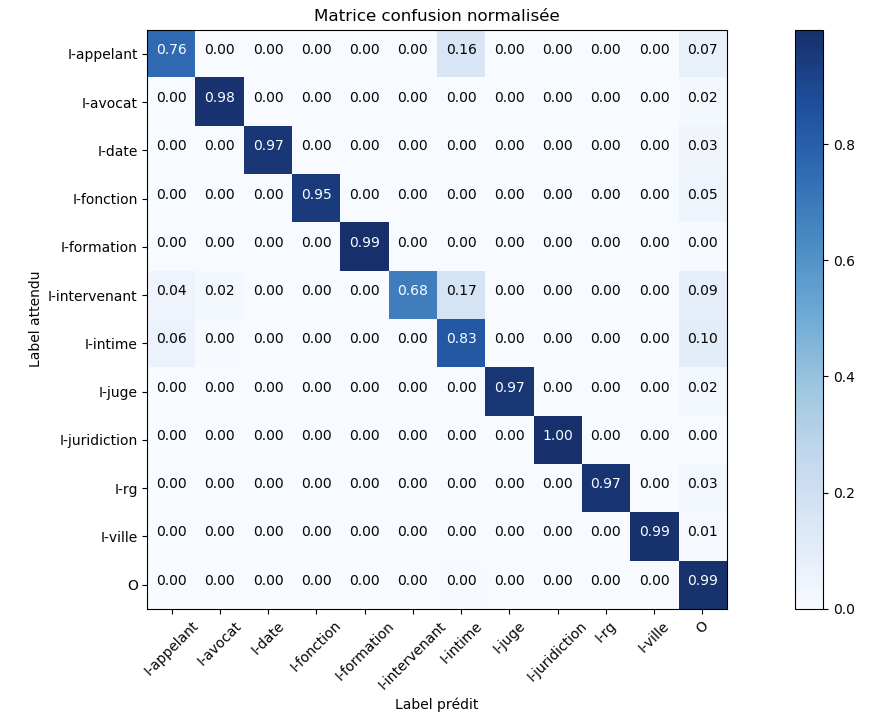
\includegraphics[width=0.8\textwidth]{confusion_matrix_entete.png}
    %\textcolor{red}{Matrices de confusion}
    \caption{Matrice de confusion entre méta-données d'entête avec le modèle CRF}
    \label{fig:structuration:matrice-confusion-entete}
\end{figure}

La proximité crée aussi des confusions entre les sections CORPS et DISPOSITIF qui se suivent (Figure \ref{fig:structuration:matrice-confusion-section}).  

\begin{figure}[h!]
	\centering
	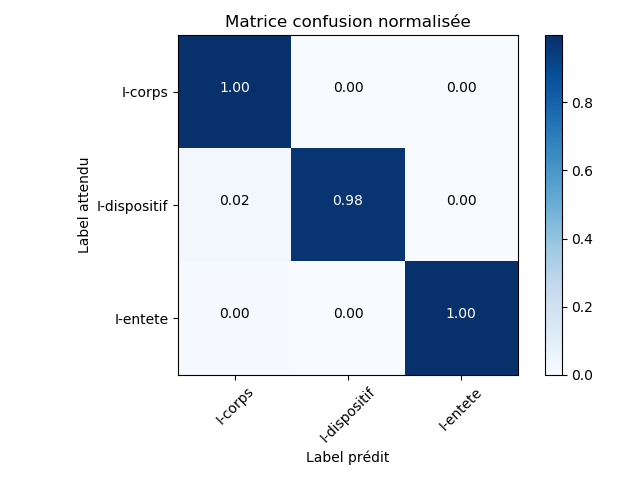
\includegraphics[width=0.8\textwidth]{confusion_matrix_section.png}
	%\textcolor{red}{Matrices de confusion}
	\caption{Matrice de confusion  avec le modèle CRF}
	\label{fig:structuration:matrice-confusion-section}
\end{figure}

\subsubsection{Redondance des mentions d'entités}
Il est aussi intéressant de remarquer que certaines entités sont répétées dans le document. Par exemple, les des parties sont mentionnées précédemment à une autre mention qui donne plus de détail sur eux. Certaines normes sont aussi citées de manière répétée et en alternant souvent les formes allongées et des longues. Malgré le fait que les mentions répétées ne sont pas identiques, de telles redondance aident à réduire le risque de manquer une entité. Cette aspect peut être exploité afin de combler l'imperfection des modèles.


\subsubsection{Impact de la quantité d'exemples annotées}
\begin{figure}[!h]
	\centering
	\begin{subfigure}[t]{0.95\textwidth}
		\centering
		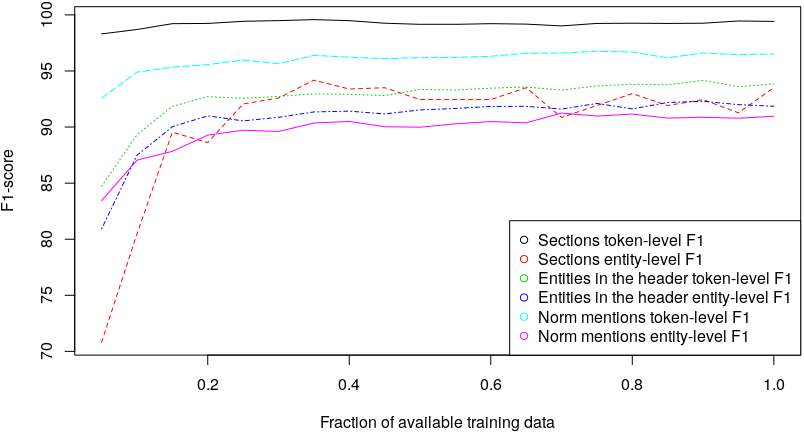
\includegraphics[width=0.75\textwidth]{lc-crf.png}
		\caption{CRF} \label{fig:structuration:learning-curves-crf}
	\end{subfigure} 
	
	\begin{subfigure}[t]{0.95\textwidth}
		\centering
		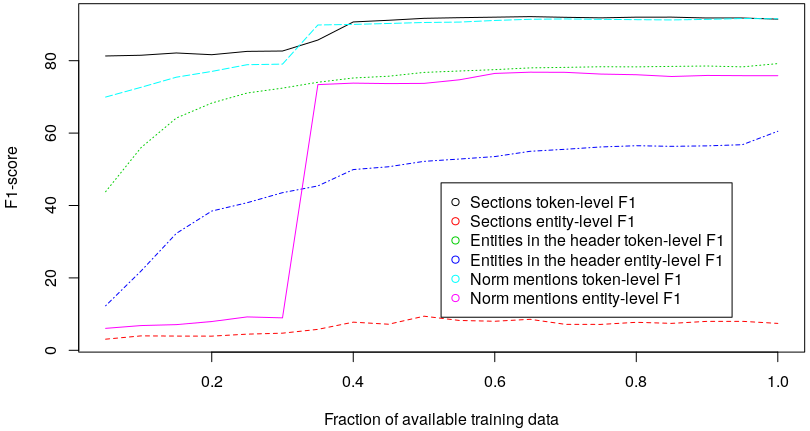
\includegraphics[width=0.75\textwidth]{lc-hmm.png}
		\caption{HMM} \label{fig:structuration:learning-curves-hmm}
	\end{subfigure}
	\caption{Courbes d'apprentissages aux niveaux élément et entité} \label{fig:structuration:learning-curves}
\end{figure}

Certaines expérimentations ont été conduites pour évaluer comment les modèles s'améliorent lorsqu'on augmente le nombre de données d'entraînement. Pour cela, nous avons calculé les performances des modèles pour de différentes taille de la base d'entraînement. Les données ont été divisées en $75\%-25\%$ pour resp. l'entraînement et le test. 20 fractions de l'ensembles d'entraînement ont été testées (de 5\% à 100\%). A chaque session entraînement-test, le même jeu de test a été utilisé pour les différentes fractions de l'ensemble d'entraînement. Les courbes d'apprentissage des modèles CRF et HMM sont représentées resp. sur les Figures \ref{fig:structuration:learning-curves-crf} et \ref{fig:structuration:learning-curves-hmm}. Il est évident que les scores F1 croissent avec plus de données d'entraînement pour les CRF et HMM, mais cette amélioration devient très faible au-delà de 60\% de données d'entraînement quelque soit la tâche. Il est possible que les exemples rajoutés à partir de là partagent la même structure qu'une majorité d'autres. Ainsi, cette étude doit être étendue à la sélection des exemples les plus utiles. \citet{raman2003exampleSelection} a démontré les avantages des algorithmes de sélection d'exemples combinés à la sélection de caractéristique pour la classification. Les mêmes méthodes sont probablement applicables à l'étiquetage de séquence.



\subsubsection{Descripteurs manuels vs. réseau de neurones}

\begin{table}[!h]
	\scriptsize
	\centering
	\begin{tabular}{|l|l|l|l|l|l|l|}
		\hline
		&               \multicolumn{3}{c}{\textbf{CRF + descripteurs manuels}} & \multicolumn{3}{|c|}{\textbf{BiLSTM-CRF}}   \\ \cline{2-7}
		& \textit{Precision} & \textit{Rappel}                     & \textit{F1} & \textit{Precision} & \textit{Rappel}      & \textit{F1} \\ \hline
		\textbf{appelant}      & 82.49              & 69.42                               & 74.72       & 80.26              & 71.53                & 75.04       \\ 
		\textbf{avocat}        & 90.15              & 89.02                               & 89.56       & 84.93              & 87.88                & 86.36       \\ 
		\textbf{date}          & 95.34              & 91.46                               & 93.12       & 95.04              & 90.79                & 92.63       \\ 
		\textbf{fonction}      & 95.87              & 95.08                               & 95.44       & 92.69              & 93.48                & 93.03       \\ 
		\textbf{formation}     & 96.91              & 91.31                               & 93.7        & 91.05              & 89.47                & 89.84       \\ 
		\textbf{intervenant}   & 51.42              & 32.71                               & 36.8        & 31.48              & 20                   & 23.11       \\ 
		\textbf{intime}        & 76.01              & 79.15                               & 77.22       & 67.7               & 75.43                & 70.83       \\ 
		\textbf{juge}          & 95.67              & 94.07                               & 94.84       & 95.44              & 95.56                & 95.46       \\ 
		\textbf{juridiction}   & 98.55              & 98.25                               & 98.33       & 97.95              & 99.22                & 98.57       \\ 
		\textbf{rg}            & 95.46              & 95.29                               & 95.27       & 91.13              & 97.26                & 93.92       \\ 
		\textbf{ville}         & 98.33              & 93.01                               & 94.71       & 91.43              & 95.34                & 93.3        \\ 
		\textbf{norme}         & 91.08              & 90.27                               & 90.67       & 91.43              & 92.65                & 92.03       \\ \hline
		\noalign{\smallskip}\hline\noalign{\smallskip}
		\textbf{Eval. globale} & 92.2               & 90.09                               & 91.12       & 89.21              & 90.43                & 89.81       \\ \hline
	\end{tabular}
	\caption{Comparaison du CRF avec descripteurs manuellement défini et le BiLSTM-CRF au niveau entité.}\label{tab:structuration:perf-bilstmcrf}
\end{table}

L'ingénierie manuelle des caractéristiques est difficile car arbitraire. Nous avons comparé les performances de nos descripteurs avec celles des réseaux de neurones qui apprennent une représentation des segments. Pour cela nous avons choisi le BiLSTM-CRF de \citet{lample2016nnner} qui fait partie des meilleures approches récentes. La comparaison a été effectuée pour la détection des entités avec le schéma d'étiquetage BIEO et une validation croisée à 9 itérations. Le BiLSTM-CRF prend entrée les plongements sémantiques Word2Vec des mots. Pour cela, nous avons entraîné des vecteurs de mots à partir d'un corpus jurisprudentiel de plus de 800K documents provenant de \url{www.legifrance.gouv.fr} avec l'implémentation\footnote{\url{https://code.google.com/archive/p/word2vec/}} de \citet{lemikolov2014word2vec}. Les vecteurs obtenus ont une dimension de 300. Etant donné que les décisions sont des documents particulièrement longs, leur contenu a été découpé en morceaux de texte dont la taille n'excède pas 300 mots. Les résultats obtenus (Tableau \ref{tab:structuration:perf-bilstmcrf}) sont assez proches. Etant donné que les descripteurs manuellement définis permettent de mieux détecter certaines entités comme les \textit{intervenants}, les \textit{avocats} ou les numéro \textit{R.G.}, et vice-versa pour les \textit{normes} ou les \textit{appelants} chez le BiLSTM-CRF, une combinaison des deux types de descripteurs pourrait améliorer les résultats actuels. On peut par exemple exploiter des modèles thématiques déduits en partitionnant (\textit{clustering}) l'ensemble des vecteurs de mots  et les utiliser comme descripteurs définis manuellement. 
 

\section{Conclusion}
\label{sec:structuration:conclusion}
L'application des modèles HMM et CRF dans le but de détecter des sections et des entités dans les décisions de justice est une tâche difficile. Ce chapitre a examiné les effets de divers aspects de la conception sur la qualité des résultats. En résumé, l'amélioration obtenue semble être assez insignifiante lorsque l'on sélectionne séparément la représentation du segment et le sous-ensemble de caractéristiques. Cependant, opter pour la bonne configuration en comparant la sélection de sous-ensembles d'entités avec diverses représentations de segment pourrait offrir une meilleure méthode. En raison de la longue période nécessaire pour rechercher le sous-ensemble de fonctionnalités optimal, il serait préférable d'utiliser un algorithme de sélection de fonctionnalités très rapide. De plus, même si les résultats s'améliorent avec la croissance de l'échantillon d'apprentissage, la mesure globale F1 semble néanmoins atteindre une limite très rapidement. Étant donné que certaines entités ne sont pas très bien détectées, il peut être avantageux d'ajouter des exemples appropriés afin de traiter ces problèmes spécifiques.

L'application des modèles pose deux difficultés majeures: l'annotation d'un nombre suffisant d'exemples et la définition de caractéristiques compatibles (c'est-à-dire pouvant être combinées pour améliorer les résultats). Les efforts d'annotation peuvent être réduits avec un système dont les performances réelles démontrent la capacité d'étiqueter correctement la plupart des entités. Il suffirait alors de vérifier manuellement ces annotations afin de corriger toute erreur commise par le système lors de nouvelles décisions à l'aide de cadres annotatifs. En ce qui concerne la définition des caractéristiques, dans la mesure où nous définissons manuellement des caractéristiques potentielles en analysant quelques documents, il est possible que ces caractéristiques ne s'intègrent pas parfaitement dans un ensemble de données différent (différents pays, différentes langues, différentes juridictions). Pour éviter les énormes efforts requis pour définir les fonctionnalités manuellement, il serait préférable d'utiliser des descripteurs automatiquement apprises à partir de corpus étiquetés ou non, comme des mots incorporés.

Dans les travaux futurs, Il serait intéressant d'achever la tâche de reconnaissance d'entités nommées. En construisant une base de connaissances, il est en effet essentiel de définir des approches de désambiguïsation et de résolution pour les entités à occurrences multiples, en plus de la correspondance des entités extraites avec des entités de référence, comme l'ont expérimenté \citet{dozier2010legalnerr} et \citet{cardellino2017legalNERCL}. 